% !TEX root = ../../../main.tex
% 来源：高中物理甲种本·第三册（电磁·光学·近代物理）
% 章节：磁场 / 磁现象的电本质~~磁性材料
% 原始文件：1.tex，行 167-183
% 类型：tikz
% ---
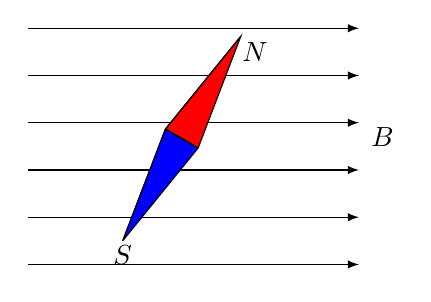
\begin{tikzpicture}[>=latex, scale=.6]
\foreach \x in {-.5,.5,...,4.5}
{
   \draw [->](-2,\x)--(5,\x);
}

\draw [rotate=60, fill=red](2.5,-.4)--(2.5,.4)--(5,0);
\draw [rotate=60, fill=blue](2.5,-.4)--(2.5,.4)--(0,0);

\draw [rotate=60](0,0)--(2.5,-.4)--(5,0)--(2.5,.4)--(0,0);
\draw [rotate=60](2.5,-.4)--(2.5,.4);

\node at (0,-.3){$S$};
\node at (2.8,4){$N$};

\node at  (5.5,2.2){$B$};
\end{tikzpicture}
